\documentclass[conference]{IEEEtran}
\IEEEoverridecommandlockouts

\usepackage[utf8]{inputenc}
\usepackage[T5]{fontenc}
\usepackage{cite}
\usepackage{amsmath,amssymb,amsfonts}
\usepackage{graphicx}
\usepackage{textcomp}
\usepackage{xcolor}
\usepackage{booktabs}
\usepackage{multirow}
\usepackage{tikz}
\usepackage{placeins}
\usepackage{float}
\usetikzlibrary{arrows.meta,positioning,shapes.geometric,fit,backgrounds}

\def\BibTeX{{\rm B\kern-.05em{\sc i\kern-.025em b}\kern-.08em
    T\kern-.1667em\lower.7ex\hbox{E}\kern-.125emX}}

\begin{document}

\title{An LLM-Augmented Stacked Ensemble for Vietnamese Emotion Recognition on Social Media}

\author{%
\IEEEauthorblockN{Nguy\~{\^e}n Gia Huy}
\IEEEauthorblockA{\textit{School of Computer Science and Engineering}\\
\textit{International University}\\
\textit{Vietnam National University}\\
Ho Chi Minh City, Vietnam\\
ITDSIU22165@student.hcmiu.edu.vn}
\and
\IEEEauthorblockN{Nguy\~{\^e}n Th\d{i} Thanh Sang\textsuperscript{$\ast$}}
\IEEEauthorblockA{\textit{School of Computer Science and Engineering}\\
\textit{International University}\\
\textit{Vietnam National University}\\
Ho Chi Minh City, Vietnam\\
nttsang@hcmiu.edu.vn}
}

\maketitle
\footnotetext[1]{$\ast$Corresponding author: nttsang@hcmiu.edu.vn}
% -----------------------------------------------------------------------
\section*{Abstract}
Fine-grained emotion recognition from Vietnamese social-media text is a difficult natural language processing problem due to the language's low-resource status and severe class
imbalance in available corpora. This paper proposes a two-stage framework for Vietnamese emotion recognition, evaluated on UIT-VSMEC, a seven-class Vietnamese social-media emotion corpus. In the first stage, we apply targeted data augmentation using Gemini-2.5-Flash via few-shot prompting, generating synthetic examples and paraphrasing existing ones for underrepresented emotion classes (Fear, Anger, Surprise). In the second stage, we construct a stacked ensemble of five heterogeneous base classifiers (PhoBERT, CafeBERT, ViBERT, Logistic Regression, LinearSVC), whose out-of-fold probability estimates are aggregated into a structured dataset and used to fine-tune a Gemma-2-9B-it meta-model with QLoRA (4-bit quantization). The full framework achieves 70.23\% accuracy, 70.22\% weighted F1, and 68.31\% macro F1 on UIT-VSMEC, surpassing the prior CNN+word2vec weighted F1 of 59.74\% and outperforming zero-shot Gemma prompting, published transformer baselines, and classical ensemble methods.

\begin{IEEEkeywords}
Vietnamese NLP, emotion recognition, data augmentation, large language models,
ensemble learning, social media
\end{IEEEkeywords}

% -----------------------------------------------------------------------
\section{Introduction}

The rapid growth of Vietnamese social-media platforms---Facebook, TikTok, Zalo---has
produced vast volumes of user-generated text carrying rich emotional signals. Mining
these signals through fine-grained Emotion Recognition (ER) yields value for market
research, opinion monitoring, and mental health screening, yet ER remains substantially
harder than coarse sentiment polarity classification. Sentiment analysis on Vietnamese
text---typically framed as a three-class task (positive, negative, neutral)---has
benefited from larger annotated corpora, mature pre-trained language models, and
relatively clear lexical polarity cues. Hybrid architectures such as PhoBERT combined
with CNN-LSTM reach over 93\% accuracy on the UIT-VSFC student-feedback corpus
\cite{nguyen2018vsfc,nguyen2018deeplearning,nguyen2025phobert}, and several deep-learning
baselines report F1 scores above 90\% on comparable polarity benchmarks. By contrast, fine-grained emotion recognition
assigns each sentence to one of seven distinct affective states (e.g., Enjoyment,
Sadness, Fear, Anger, Disgust, Surprise, Other), where labels are linguistically
subtler, more context-dependent, and frequently confounded in informal social-media
writing \cite{hayatu2025emotion}. On UIT-VSMEC, the best reported result from the original benchmark study
reaches only 59.74\% weighted F1 using CNN with word2vec embeddings
\cite{ho2020emotion}---a gap of more than 30 percentage points relative to polarity
systems. Subsequent monolingual BERT models have narrowed but not closed this divide,
indicating that scaling pre-training alone is insufficient for reliable fine-grained
Vietnamese emotion classification.

Two interconnected obstacles drive this gap. First, Vietnamese is a low-resource
language \cite{duong2021review,mai2025neuesc}: annotated datasets are scarce, and existing corpora
tend to be small. Second, UIT-VSMEC suffers from pronounced class imbalance: the
dominant label \textit{Enjoyment} constitutes roughly 28\% of the training set, whereas
minority emotions such as \textit{Surprise} ($\sim$4.5\%) and \textit{Anger}
($\sim$6.9\%) are severely underrepresented. Together, these constraints limit the
robustness and generalization of individual classifiers.

We address both obstacles with a unified two-stage framework. In the first stage, we
exploit the generative capabilities of a large language model (LLM), specifically
Gemini-2.5-Flash \cite{ding2024augmentation}, to perform targeted data augmentation
for minority emotion classes using 10-shot prompting. In the second stage, we build a
stacked ensemble whose base predictions are aggregated into a structured dataset and
used to fine-tune a Gemma-2-9B-it meta-model with parameter-efficient QLoRA.

The main contributions of this paper are:
\begin{enumerate}
  \item An LLM-based augmentation protocol that generates and paraphrases Vietnamese
        social-media sentences for minority emotion classes, demonstrably improving
        minority-class F1 scores with a controlled 10-shot prompting strategy.
  \item A stacked ensemble framework that combines Vietnamese BERT models and
        classical TF-IDF classifiers with a QLoRA-fine-tuned Gemma meta-learner,
        achieving accuracy-weighted aggregation of diverse classifier signals.
  \item Empirical validation of the proposed Vietnamese emotion recognition
        framework on UIT-VSMEC, establishing a new state-of-the-art of
        70.23\% accuracy, 70.22\% weighted F1, and 68.31\% macro F1 and
        outperforming zero-shot LLM prompting, published BERT baselines, and
        prior ensemble methods.
\end{enumerate}

% -----------------------------------------------------------------------
\section{Related Work}

\subsection{Vietnamese Emotion Recognition}

Ho et al.\ \cite{ho2020emotion} introduced UIT-VSMEC, a 6,927-sentence seven-class
corpus, establishing a CNN+word2vec baseline of 59.74\% weighted F1. Nguyen and
Nguyen \cite{nguyen2020exploiting} reached 64.40\% through multi-label regression
with preprocessing and key-clause extraction. Pre-trained transformers further
narrowed the gap: PhoBERT \cite{nguyen2020phobert} underpins hybrid
CNN-LSTM architectures that achieve 93.24\% accuracy on the polarity task
\cite{nguyen2025phobert}, but the fine-grained ER on informal social-media text remains
harder. CafeBERT \cite{do2024vlue} (XLM-RoBERTa trained on Vietnamese Wikipedia and
news) reports 66.12\% F1 on VSMEC; ViSoBERT \cite{nguyen2024visobert} reaches
68.37\% weighted F1; and a GRU--CNN--BiLSTM--LSTM ensemble \cite{huynh2020ensemble}
attains 65.79\% macro F1. Despite these advances, minority emotions such as Fear,
Anger, and Surprise remain difficult to classify and leave room for data-centric and
ensemble improvements.

\subsection{LLM-based Augmentation and Ensemble Methods}

Ding et al.\ \cite{ding2024augmentation} survey LLM-driven data creation and
co-annotation, noting risks of contamination and model collapse. Ubani et al.\
\cite{ubani2023zeroshotdataaug} show zero-shot ChatGPT generation outperforms EDA
and back-translation on SST-2 and SNIPS; Whitehouse et al.\
\cite{whitehouse2023llmaug} extend LLM augmentation to cross-lingual settings; \"{U}veges and Ring
\cite{uveges2025synthetic} confirm 10-shot LLM prompting yields macro-F1 gains for
underrepresented emotion classes. However, prior work treats the LLM as an offline
generator only, and prompt design for fine-grained Vietnamese emotion categories
remains underexplored. On the ensemble side, Thin et al.\ \cite{thin2024ensemble}
obtain 94.03\% weighted F1 on VSFC \cite{nguyen2018vsfc} via soft-voting over five Vietnamese transformers;
Niimi \cite{niimi2025ensemble} unifies multiple LLM inferences through bagging and
weighted averaging. Thin et al.\ \cite{thin2024prompt} further evaluate zero- and
few-shot LLM prompting for Vietnamese sentiment, while Zhang and Han
\cite{zhang2025commonsense} integrate commonsense knowledge into fine-grained
aspect-level analysis, highlighting leakage risks with generative models. Our work
extends these directions by using Gemini-2.5-Flash for targeted augmentation and as a
QLoRA-fine-tuned meta-learner over heterogeneous ensemble signals.

\FloatBarrier
% -----------------------------------------------------------------------
\section{Methodology}

\begin{figure}[!t]
\centering
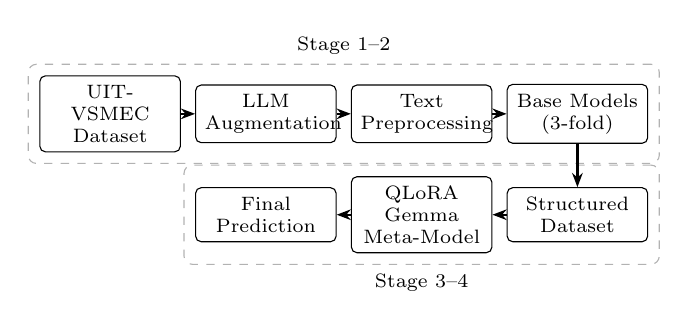
\begin{tikzpicture}[
  node distance=0.32cm and 0.18cm,
  box/.style={draw, rounded corners=2pt, align=center, font=\scriptsize,
              minimum height=0.58cm, text width=1.55cm, fill=white},
  arr/.style={-{Stealth[length=1.8mm]}, thick},
  grp/.style={draw=gray!60, dashed, rounded corners=3pt, inner sep=4pt}
]
  % Top row
  \node[box] (data)    {UIT-VSMEC\\Dataset};
  \node[box, right=of data]  (aug)     {LLM\\Augmentation};
  \node[box, right=of aug]   (prep)    {Text\\Preprocessing};
  \node[box, right=of prep]  (base)    {Base Models\\(3-fold)};

  % Bottom row
  \node[box, below=0.55cm of base] (meta)  {Structured\\Dataset};
  \node[box, left=of meta]         (lora)  {QLoRA Gemma\\Meta-Model};
  \node[box, left=of lora]         (pred)  {Final\\Prediction};

  % Arrows top row
  \draw[arr] (data) -- (aug);
  \draw[arr] (aug)  -- (prep);
  \draw[arr] (prep) -- (base);

  % Bend down
  \draw[arr] (base.south) -- (meta.north);

  % Bottom row (right to left)
  \draw[arr] (meta) -- (lora);
  \draw[arr] (lora) -- (pred);

  % Grouping backgrounds
  \begin{pgfonlayer}{background}
    \node[grp, fit=(data)(aug)(prep)(base), label=above:{\scriptsize Stage 1--2}] {};
    \node[grp, fit=(meta)(lora)(pred), label=below:{\scriptsize Stage 3--4}] {};
  \end{pgfonlayer}
\end{tikzpicture}
\caption{Proposed pipeline: augmentation and preprocessing feed the base models; their
cross validation probabilities form a structured dataset for QLoRA Gemma fine-tuning.}
\label{fig:pipeline}
\end{figure}

This study proposes an end-to-end pipeline for processing Vietnamese social media data and recognizing emotions in sentences, as illustrated in Fig.~\ref{fig:pipeline}. It consists of four stages: LLM data augmentation, text preprocessing, base classifier training with cross validation stacking, and meta-model fine-tuning.

\subsection{LLM-based Data Augmentation}

\begin{figure}[H]
\centering
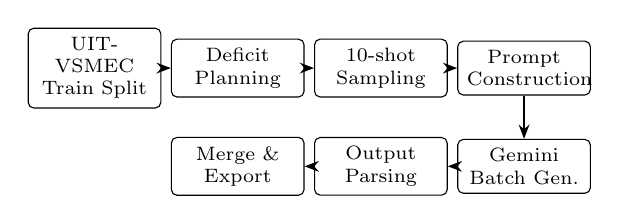
\begin{tikzpicture}[
  node distance=0.28cm and 0.12cm,
  box/.style={draw, rounded corners=2pt, align=center, font=\scriptsize,
              minimum height=0.55cm, text width=1.45cm, fill=white},
  arr/.style={-{Stealth[length=1.8mm]}, thick}
]
  \node[box] (split)  {UIT-VSMEC\\Train Split};
  \node[box, right=of split]  (deficit) {Deficit\\Planning};
  \node[box, right=of deficit] (sample) {10-shot\\Sampling};
  \node[box, right=of sample]  (prompt) {Prompt\\Construction};
  \node[box, below=0.55cm of prompt] (gemini) {Gemini\\Batch Gen.};
  \node[box, left=of gemini]   (parse)  {Output\\Parsing};
  \node[box, left=of parse]    (merge)  {Merge \&\\Export};

  \draw[arr] (split)   -- (deficit);
  \draw[arr] (deficit) -- (sample);
  \draw[arr] (sample)  -- (prompt);
  \draw[arr] (prompt.south) -- (gemini.north);
  \draw[arr] (gemini)  -- (parse);
  \draw[arr] (parse)   -- (merge);
\end{tikzpicture}
\caption{Synthetic data creation pipeline for minority-class augmentation.}
\label{fig:aug_pipeline}
\end{figure}

UIT-VSMEC exhibits a 6.4:1 imbalance between the most and least frequent classes. We
address this by prompting Gemini-2.5-Flash \cite{ding2024augmentation} via the Gemini chat interface to generate additional training examples for the
three most underrepresented emotions: Fear, Anger, and Surprise. Two complementary
strategies are applied: (i)~\textit{generated}---the model synthesizes entirely new
Vietnamese sentences conditioned on an emotion label and 10 randomly sampled in-context
examples, creating novel scenarios not present in the original corpus;
(ii)~\textit{paraphrased}---the model rewrites existing annotated sentences
with linguistic variation while preserving the target emotion and original semantics.
Each class is augmented to a target of 1,500 examples per strategy. Augmentation operates
on the raw training split before any preprocessing.
Fig.~\ref{fig:aug_pipeline} shows the six-stage pipeline.

The pipeline operates as follows:
\begin{enumerate}
  \item \textbf{Deficit planning.} For each minority class, the minimum number of examples required is 1,500. Other classes with numbers exceeding this target will be ignored
  \item \textbf{10-shot sampling.} Ten in-class sentences are sampled uniformly at
        random (with replacement when the class has fewer than ten examples) to form
        the few-shot context.
  \item \textbf{Prompt construction.} A system message and structured human message
        are assembled from the selected template (generated or paraphrased).
  \item \textbf{Batch generation.} The prepared prompts are sent to
        Gemini-2.5-Flash in groups of up to 50 at a time, so many candidate
        sentences can be produced in parallel rather than one by one. We set
        generation temperature to 0.9 to encourage varied wording across outputs
        \cite{li2025temperature}, and apply a frequency penalty of 0.5 so the
        model is less likely to repeat the same phrases. Each response yields a
        batch of new Vietnamese sentences for the target emotion.
  \item \textbf{Output parsing.} Each response is parsed line by line; only lines that follow the expected numbered format (a sequence number, a generated sentence, and a reference to the few-shot example it was based on) are kept. Lines that do not match this pattern are discarded.
  \item \textbf{Merge and export.} Accepted sentences are tagged
        (marked as augmented with their source strategy), trimmed to the exact deficit, and
        concatenated with the original training split.
\end{enumerate}

\begin{table}[H]
\caption{Prompt design comparison: generated vs.\ paraphrased strategy}
\label{tab:prompt_design}
\centering
\footnotesize
\begin{tabular}{@{}p{0.18\columnwidth}p{0.33\columnwidth}p{0.33\columnwidth}@{}}
\toprule
 & \textbf{Generated} & \textbf{Paraphrased} \\
\midrule
System role &
  VN social-media expert; express target emotion only &
  Gen-Z social-media expert; preserve meaning, tone, intent \\
\midrule
Human task &
  Synthesize NEW sentences for the target emotion (in English and Vietnamese) &
  Rewrite sentences preserving SAME meaning and emotion \\
\midrule
Key constraints &
  Natural VN style; length mix (5--10 / 10--20 / 20+ words); no other emotions &
  Semantic equivalence mandatory; no new facts or intensity; preserve negation and intensifiers \\
\midrule
Output format &
  \multicolumn{2}{p{0.62\columnwidth}}{Numbered lines: sequence number, generated sentence, and example reference} \\
\bottomrule
\end{tabular}
\end{table}

\begin{table}[H]
\caption{Examples of augmented sentences by strategy}
\label{tab:gen_examples}
\centering
\footnotesize
\begin{tabular}{@{}lp{0.18\columnwidth}p{0.20\columnwidth}l@{}}
\toprule
Strategy & Original & Output & Emotion \\
\midrule
Gen. & per không cho anh đi tập đâu nha mất bồ như chơi &
  Cái cảm giác bị bỏ rơi nó ám ảnh tui ghê lắm. & Fear \\[2pt]
Gen. & sao mà mặt boss có thể gian phản diện đến thế nhỉ &
  Sao nhìn cái mặt của nhân vật phản diện nó gian manh vậy ta. & Surprise \\[2pt]
Gen. & per bất hạnh thật tao với mày mua bánh ăn chung đi &
  Đời tôi khốn nạn lắm rồi, đừng ai làm phiền nữa. & Anger \\[2pt]
Para. & sợ ngỗng còn hơn sợ chó :))) &
  Thà sợ chó còn hơn sợ ngỗng :))) & Fear \\[2pt]
Para. & vl :)) còn đút tay túi áo ?? &
  Trời đất ơi, còn đút tay vào túi áo nữa hả? & Surprise \\[2pt]
Para. & dẹp . đéo lưu luyến . &
  Thôi đi. Đéo cần vương vấn gì hết. & Anger \\
\bottomrule
\end{tabular}
\end{table}

\subsubsection{Prompt Design}

Both strategies share the same two-part prompt template structure: a
\textit{system message} that constrains style and emotion fidelity, and a
\textit{human message} that supplies the emotion label, its Vietnamese description,
and 10 few-shot examples. Table~\ref{tab:prompt_design} summarises the key
differences; Table~\ref{tab:gen_examples} shows representative outputs for both
strategies (Gen. for Generated and Para. for Paraphrased). The shared output format requires each line to be numbered and include a reference to the few-shot example it was based on, enabling consistent parsing.

\subsection{Text Preprocessing}

Vietnamese social-media text is noisy: users mix emojis, keyboard emoticons, slang, and
short forms that carry strong emotional meaning. If these signals are removed too early,
models may lose useful cues. Following practices similar to prior Vietnamese social-media
emotion work \cite{nguyen2020exploiting,duong2021review}, we therefore apply a shared
cleaning pipeline to the training, validation, and test splits after augmentation.

Each sentence is cleaned in four steps. First, a curated dictionary of 116 emoji-to-Vietnamese
mappings replaces Unicode emojis with short descriptive phrases (e.g., ``vui vẻ'' for
happy faces and ``buồn bã'' for sad faces); unmatched emojis are then removed with a
Unicode regex filter. Second, 39 text emoticons such as \texttt{:))}, \texttt{:(}, and
\texttt{T\_T} are mapped to Vietnamese words, with longer patterns matched first to avoid
partial replacements. Third, 95 common internet abbreviations are expanded at the word
level (e.g., \textit{ko}/\textit{k}/\textit{hok}, all meaning \textit{không};
\textit{dc}/\textit{đc}, meaning \textit{được}). Fourth, URLs and HTML tags are
stripped, non-Vietnamese characters are replaced with spaces while diacritics and basic
punctuation are kept, repeated punctuation is collapsed, and whitespace is normalized.

After cleaning, duplicate sentences are removed so repeated content does not bias training.
Stopwords are intentionally kept. Function words such as \textit{không} (negation) and
\textit{rất} (intensifier) often change emotion meaning, and BERT-style encoders can use
these tokens through self-attention \cite{nguyen2020phobert,do2024vlue}.

\subsection{Base Classifiers}

Five heterogeneous base classifiers are trained with stratified 3-fold cross-validation,
each producing probability vectors across the seven emotion classes:

\begin{itemize}
  \item \textbf{PhoBERT-v2} \cite{nguyen2020phobert}: pre-trained on Vietnamese Wikipedia
        and news; fine-tuned for 20 epochs.
  \item \textbf{CafeBERT} \cite{do2024vlue}: a Vietnamese BERT variant from the VLUE
        benchmark; best single-model accuracy on VSMEC.
  \item \textbf{ViBERT}: a Vietnamese BERT model further pre-trained on Vietnamese text.
  \item \textbf{Logistic Regression}: TF-IDF features, L2 regularization \cite{bollapragada2018lbfgs}.
  \item \textbf{LinearSVC}: TF-IDF features, wrapped in a probability calibration layer
        to produce class probability estimates.
\end{itemize}

Each model is also refitted on the full training set to produce validation and test
probability arrays. Classifier metrics are stored as JSON artifacts.

\subsection{Stacked Ensemble with LLM Meta-Model}

\textbf{Weights and structured dataset.}
Each base model is assigned a weight proportional to its validation-set accuracy: a model's weight equals its individual accuracy divided by the sum of all five models' accuracies. This produces a set of normalized weights that sum to one, so higher-performing models contribute more to the final prediction.
For each training example, a structured input is then assembled that combines the original sentence, each base model's predicted probability distribution over the seven emotion classes, and the overall weighted-average prediction. This combined representation captures both each model's individual confidence and the degree of disagreement across models.

\textbf{QLoRA fine-tuning.}
Gemma-2-9B-it serves as the meta-learner. The model is
fine-tuned with QLoRA (4-bit NF4 quantization, rank-16 adapters) using completion-only
cross-entropy loss on the emotion label as the target output. Training
uses the structured training dataset built from out-of-fold predictions (unbiased by construction), which
mitigates information leakage into the meta-model \cite{sasso2022transfer}. At inference, the model generates the
emotion label conditioned on the structured meta-prompt for each test example.

% -----------------------------------------------------------------------
\section{Experiments}

\subsection{Dataset and Splits}

UIT-VSMEC \cite{ho2020emotion} contains 6,927 human-annotated sentences drawn from
Vietnamese social-media platforms, covering seven emotion labels: Enjoyment, Sadness,
Fear, Anger, Disgust, Surprise, and Other. We follow the standard 8:1:1 split protocol,
yielding approximately 5,548 training, 686 validation, and 693 test sentences after
preprocessing. The training set is augmented to 1,500 examples per class for the minority
classes before preprocessing.

\subsection{Baselines and Evaluation}

We evaluate on the two following experimental conditions. Evaluation metrics are accuracy, weighted F1 (W-F1), and macro F1.

\textbf{Augmentation ablation.} CafeBERT is trained on three versions of the training
data---original, paraphrased-augmented, and generated-augmented---and evaluated on the
held-out test set using accuracy, weighted F1, and per-class F1 for the three minority
emotions (Fear, Anger, Surprise).

\textbf{Ensemble comparison.} Table~\ref{tab:ensemble} compares the proposed stacked
ensemble against (i)~Gemma-2-9B-it zero-shot prompting on the same structured
meta-prompts; (ii)~published monolingual and multilingual transformer results on
UIT-VSMEC (CafeBERT and XLM-RoBERTa-Large from VLUE \cite{do2024vlue}, ViSoBERT
\cite{nguyen2024visobert}); (iii)~the MLR pipeline with preprocessing and key-clause
extraction \cite{nguyen2020exploiting}; and (iv)~the GRU--CNN--BiLSTM--LSTM neural
ensemble \cite{huynh2020ensemble}. For context, the original UIT-VSMEC benchmark
CNN+word2vec baseline \cite{ho2020emotion} reached 59.74\% weighted F1 but is omitted
from Table~\ref{tab:ensemble} because it predates the transformer-centric comparison
protocol used in our evaluation.


\FloatBarrier
% -----------------------------------------------------------------------
\section{Results and Analysis}

\subsection{Impact of LLM Augmentation}

Table~\ref{tab:augmentation} reports CafeBERT performance across the three training
conditions.

\begin{table}[H]
\caption{Impact of LLM augmentation on CafeBERT (UIT-VSMEC test set)}
\label{tab:augmentation}
\centering
\begin{tabular}{@{}lccccc@{}}
\toprule
Training Data & Acc. & W-F1 & Fear & Anger & Surprise \\
\midrule
Original      & 0.6344 & 0.628 & 0.67 & 0.38 & 0.60 \\
Paraphrased   & 0.6676 & 0.6682 & 0.67 & 0.42 & 0.61 \\
\textbf{Generated}    & \textbf{0.6703} & \textbf{0.671} & \textbf{0.68} & \textbf{0.46} & \textbf{0.61} \\
\bottomrule
\end{tabular}
\end{table}

Both augmentation strategies yield consistent improvements. The generated
data condition produces the largest gains, raising accuracy from 63.44\% to 67.03\%
and weighted F1 from 62.8\% to 67.1\%. Minority-class gains are particularly pronounced:
Anger F1 rises from 38\% to 46\% (a gain of 8 percentage points), confirming that
synthetic generation effectively addresses the most severely imbalanced classes. Fear and
Surprise also improve, though more modestly, reflecting their lower initial imbalance.
Paraphrasing yields intermediate improvements, suggesting that linguistic variation alone
is beneficial but less impactful than generating entirely new examples.
Table~\ref{tab:synthetic_quality} further analyses the quality of the generated sentences.

\begin{table}[H]
\caption{Quality of LLM-generated training sentences (5,010 synthetic vs.\ 5,548 original)}
\label{tab:synthetic_quality}
\centering
\footnotesize
\begin{tabular}{@{}lcc@{}}
\toprule
Metric & Original & Generated \\
\midrule
Overall fidelity score    & ---   & 0.776 \\
Distinct-2                & 0.593 & 0.451 \\
Distinct-3                & 0.930 & 0.786 \\
Mean sentence length (chars) & 56.0 & 51.0 \\
Train--test leakage (exact / near) & --- & 0 / 0 \\
Emotion distribution KL div. & --- & 0.164 \\
\bottomrule
\multicolumn{3}{@{}l}{\footnotesize Fidelity = mean of stat, distribution, label, and correlation similarity.} \\
\end{tabular}
\end{table}

Zero exact and near-duplicate test-set overlap confirms no evaluation leakage in the
synthetic corpus. An overall fidelity score of 0.776 shows that generated text is
statistically close to original social-media sentences; the KL divergence of 0.164 reflects
intentional upsampling of minority classes, not a quality failure. Lower Distinct-2/3
values reveal moderate lexical repetition from 10-shot conditioning, yet generated data
still outperforms paraphrasing because novel scenarios expand minority-class coverage
more than surface variation alone.

\FloatBarrier
\subsection{Ensemble Performance}

\begin{table}[H]
\caption{Performance comparison of ensemble learning methods and baselines on UIT-VSMEC
(test set). Published transformer rows follow VLUE/ViSoBERT benchmark settings.}
\label{tab:ensemble}
\centering
\footnotesize
\begin{tabular}{@{}lccc@{}}
\toprule
Method & Acc. & W-F1 & M-F1 \\
\midrule
\textbf{Proposed (stacked + QLoRA Gemma)} & \textbf{0.7023} & \textbf{0.7022} & \textbf{0.6831} \\
Gemma zero-shot (ours)                    & 0.6864 & 0.6809 & --- \\
MLR + preprocessing \cite{nguyen2020exploiting} & 0.6436 & 0.6440 & --- \\
CafeBERT \cite{do2024vlue}                & ---    & 0.6612 & --- \\
ViSoBERT \cite{nguyen2024visobert}        & 0.6810 & 0.6837 & --- \\
XLM-RoBERTa-Large \cite{do2024vlue}        & 0.6137 & 0.6020 & --- \\
GRU--CNN--BiLSTM--LSTM \cite{huynh2020ensemble} & --- & --- & 0.6579 \\
\bottomrule
\multicolumn{4}{@{}l}{\footnotesize W-F1: weighted F1;\enspace M-F1: macro F1;\enspace ---: not reported.} \\
\end{tabular}
\end{table}

Table~\ref{tab:ensemble} reports the full UIT-VSMEC benchmark comparison. The proposed
framework achieves 70.23\% accuracy and 70.22\% weighted F1, establishing a new
state-of-the-art and surpassing CNN+word2vec \cite{ho2020emotion} by over 10 percentage points in weighted F1.

A 2.13 percentage-point gain in weighted F1 over Gemma zero-shot (70.22\% vs 68.09\%) confirms that QLoRA fine-tuning on
the structured dataset yields a meaningful gain beyond zero-shot LLM inference.
The best augmented single model (CafeBERT, 67.10\% W-F1) trails the full ensemble by
3.1 percentage points in weighted F1 (67.10\% vs 70.22\%), showing that the meta-learner successfully integrates heterogeneous BERT
and TF-IDF signals beyond any individual classifier.

% -----------------------------------------------------------------------
\section{Conclusion}

\subsection{Summary}

This paper proposed a two-stage framework for Vietnamese social-media emotion
recognition: Gemini-2.5-Flash augmentation for minority classes, followed by a
five-model stacked ensemble with a QLoRA-fine-tuned Gemma-2-9B-it meta-learner.

In the first stage, few-shot LLM augmentation consistently improved CafeBERT's
performance across all three underrepresented emotion categories. Generated synthetic
data---new sentences conditioned on 10 in-context examples---outperformed
paraphrasing, raising weighted F1 from 62.8\% to 67.1\% and increasing Anger F1 by
8 percentage points (38\% to 46\%). A fidelity analysis confirmed that the synthetic
corpus is statistically plausible (overall fidelity score 0.776, zero test-set leakage),
establishing that new scenario coverage matters more than mere surface variation.

In the second stage, stacking heterogeneous BERT and TF-IDF signals through a
QLoRA-fine-tuned meta-model produced a new state-of-the-art on UIT-VSMEC:
70.23\% accuracy, 70.22\% weighted F1, and 68.31\% macro F1, exceeding the
original CNN+word2vec benchmark by over 10 percentage points \cite{ho2020emotion}.
The full ensemble surpassed zero-shot Gemma prompting by 2.13 percentage points in weighted F1
and the best augmented single model (CafeBERT) by approximately 3.1 percentage points in weighted F1,
demonstrating that QLoRA meta-learning over structured ensemble signals yields
meaningful gains beyond either component alone. Together, these results confirm that
LLMs are effective both as offline data generators and as inference-time meta-learners
in low-resource, class-imbalanced Vietnamese NLP.

\subsection{Future Work}

Future work will explore the following directions:

\begin{enumerate}

  \item \textbf{Cross-dataset and cross-domain generalization.}
        Future work should evaluate the framework on related Vietnamese NLP tasks
        (aspect-level sentiment, hate-speech detection, multi-label corpora) to verify
        that LLM augmentation and stacked ensembling generalize beyond fine-grained
        emotion recognition.

  \item \textbf{Automated quality validation for synthetic data.}
        The moderate Distinct-2/3 scores observed in Table~\ref{tab:synthetic_quality}
        call for automated filtering before synthetic examples enter training: candidate
        filters include perplexity thresholds, emotion-consistency scoring via a held-out
        classifier, semantic-similarity caps relative to near-duplicates, and LLM-as-judge
        fluency checks. The goal is to retain minority-class coverage gains while improving
        lexical diversity and reducing formulaic patterns.

  \item \textbf{Dynamic, uncertainty-aware ensemble weighting.}
        The fixed accuracy-based weighting scheme ignores per-example
        prediction confidence and inter-model disagreement. Replacing them with
        uncertainty-derived weights---computed from prediction entropy or calibrated
        confidence scores---may improve macro F1 on minority classes where static weights
        tend to favor majority-class-dominant models.

  \item \textbf{Efficiency and deployability.}
        The current QLoRA meta-model requires substantial GPU memory at both
        training and inference time. Future work should investigate distilling the
        Gemma meta-learner into a smaller classifier or replacing it with a
        lightweight stacking head, making the framework practical for deployment
        in resource-constrained environments without sacrificing the gains from
        structured dataset from ensemble predictions.

\end{enumerate}

% -----------------------------------------------------------------------
\bibliographystyle{IEEEtran}
\bibliography{references}

\end{document}
